%!TEX root = report.tex
\section{Generating Current Timetable}
\label{sec:current_timetable_generation}

\begin{itemize}
  \item data collection
  \item data storing
  \item data processing
  \item DB optimisation
  \item python scripts and SQLs
  \item resulting table name and schema
\end{itemize}

\subsection{Collecting Bus Arrival Times}
\label{sec:collecting_arrival_times}

\par We collect bus arrival data for analysis from the live bus arrivals API. The base URL used in this project was \url{http://countdown.api.tfl.gov.uk/interfaces/ura/stream_V1}.

\par We supplied the following parameters which specify the fields returned by the \acrshort{api}.

\begin{itemize}
  \item \textit{StopID} This is the alphanumeric identifier of a bus stop. It is also known as stop\_code\_lbsl.
  \item \textit{LineName} This is the route number that is displayed on the front of the bus on any publicity advertising the route.
  \item \textit{VehicleID} The unique identifier of the vehicle.
  \item \textit{TripID} The identifer of the specific trip that the prediction is for.
  \item \textit{EstimatedTime} This is the predicted time of arrival for the vehicle at a specific stop.
  \item \textit{ExpireTime} This is the time at which the corresponding prediction is no longer valid and should stop being displayed.
\end{itemize}

\par The resulting query URL is \sloppy \url{http://countdown.api.tfl.gov.uk/interfaces/ura/stream_V1?ReturnList=StopID,LineName,VehicleID,TripID,EstimatedTime,ExpireTime}.

\par Each data entry contains an estimated arrival time for each bus journey at a given bus stop. This estimated arrival time is stored in the database via an UPDATE statement, which ensures that only the latest estimated arrival times per journey per bus stop are stored. To avoid having data being overwritten, only the entries that have been changed in the recent 10 minutes can be updated. This has been achieved through running a daemon process written in python on a virtual host. Table \ref{table:delay_arrivals_schema} shows the schema for arrivals table.

\begin{table}
\centering
\begin{tabular}{@{}llr@{}} \toprule
Column Name & Type & Default \\ \midrule
id(Primary) & int(11) & Auto Increment \\
stop\_code\_lbsl & varchar(64) &  \\
route & varchar(64) &  \\
vehicle\_id & varchar(64) & \\
trip\_id & varchar(64) & \\
arrival\_date & date &  \\
arrival\_time & timestamp & NULL \\
expire\_time & timestamp & NULL \\
recorded\_time & timestamp & Current Timestamp \\ \bottomrule
\end{tabular}
\caption{delay\_arrivals Table Schema}
\label{table:delay_arrivals_schema}
\end{table}

\subsubsection{Assumption}
We assume that the actual bus arrival time is the midpoint between the last estimated arrival time, and the system time when the clear signal (\textit{ExpireTime} = 0) is received.

\subsection{Neighbouring Stops}
\label{sec:bus_stop_locations_routes}
We imported the bus sequences into the delay\_bus\_sequences table (Table \ref{table:delay_bus_sequences})

\begin{table}
\centering
\begin{tabular}{@{}llr@{}} \toprule
Column Name & Type & Comments\\ \midrule
id(Primary Key) & int(11)  & Auto Increment\\
route & varchar(64) &  The route name\\
run & int(11) & The route direction\\
sequence & int(11) & The sequence of the bus stop in the route\\
stop\_code\_lbsl & varchar(64) & The internal bus stop identifier\\
bus\_stop\_code & varcher(64) & The public code for the bus stop\\
naptan\_atco & varchar(64) & The national identifier of the bus stop\\
stop\_name & varchar(64) & The name of the bus stop\\ \bottomrule
\end{tabular}
\caption{delay\_bus\_sequences Table Schema}
\label{table:delay_bus_sequences}
\end{table}
 \todo[inline, color=cyan]{Question: Can I skip some columns of the table schema, as those columns have not been used in the project, but just storing as reference for now?}
\par Additionally, we extracted information on all pairs of neighbouring bus stops and the routes that serve between them. We save this information in the delay\_neighbours table (Table \ref{table:delay_neighbours}). See sample data in Table \ref{table:sample_neighbours_view}.

\begin{table}
\centering
\begin{tabular}{@{}llr@{}} \toprule
Column Name & Type & Comments\\ \midrule
id(Primary Key) & int(11)  & Auto Increment\\
route & varchar(64) & The bus route \\
start\_stop & varchar(64) & The stop\_code\_lbsl for the start stop\\
end\_stop & varcher(64) & The stop\_code\_lbsl for the end stop\\ \bottomrule
\end{tabular}
\caption{delay\_neighbours Table Schema}
\label{table:delay_neighbours}
\end{table}

\begin{table}
\centering
\begin{tabular}{@{}llrr@{}} \toprule
id & route & start\_stop & end\_stop \\ \midrule
18433 & 30 & 10002 & 11469 \\
44878 & N19 & 10002 & 11469 \\
47128 & N41 & 10002 & 29772 \\
8653 & 19 & 10002 & 11469 \\ \bottomrule
\end{tabular}
\caption{Sample data in delay\_neighbours Table}
\label{table:sample_neighbours_view}
\end{table}

\subsection{Finding the average travel time between neighbouring stops}
\todo[inline] {update this part}
\par To experiment with the queries, we selected one pair of the neighbouring stops (10002, 11469), and listed the time required to travel from stop 10002 to stop 11469 by finding the difference in arrival times for each journey. Sample entries of this list is shown in Figure \ref{fig:journey_time_10002}.

\begin{figure}
\centering
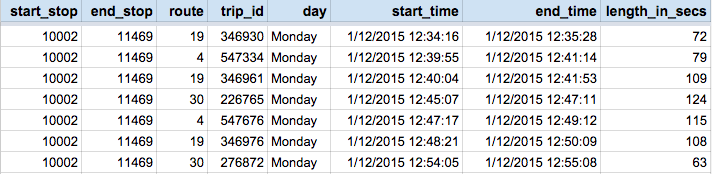
\includegraphics[width=0.7\textwidth]{figures/journey_time_10002.png}
\caption{\label{fig:journey_time_10002} List of journey time from stop 10002 to stop 11469}
\end{figure}

\par We then calculated the average journey time required to travel from 10002 to 11469 for each hour in each week of the day. This information is stored as a timetable, which would be used for further analysis.

\par Figure\ref{fig:timetable_10002} shows the timetable generated. Each cell indicates the average journey time required to travel from stop 10002 to stop 11469 at a give hour of a give week of day. The \textbf{NULL} values are due to a current databases performance issue. This will be resolved later.

\begin{figure}
\centering
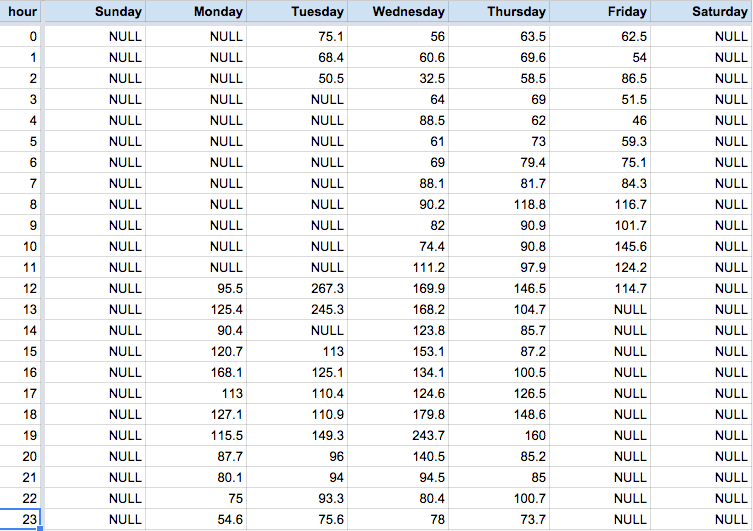
\includegraphics[width=0.9\textwidth]{figures/timetable_10002.png}
\caption{\label{fig:timetable_10002} Average journey time in seconds from stop 10002 to stop 11469 for each hour of each day of week}
\end{figure}

\par We plan to construct a timetable this way for each pair of the neighbouring bus stop.

\subsection{Negative Travel Time Filter}
\par In the travel\_time\_log generated, there were trips between two neighbouring stops with negative travel times, such as the entry shown in Table \ref{table:travel_time_log_negative}.

\begin{table}
\centering
\begin{tabular}{@{}lllllr@{}} \toprule
Start Stop & End Stop & Route & Start Time & End Time & Travel Time(sec) \\ \midrule
9326 & 15552 & W13 & 14:53:18 & 14:52:14 & -64 \\ \bottomrule
\end{tabular}
\caption{Travel Time Log Entry with Negative Travel Time}
\label{table:travel_time_log_negative}
\end{table}

\par This was because when we performed the join of the arrivals table, there was a more recent update on the arrival times for the start stop, whereas the arrival times of end stop had not been updated. In Table \ref{table:negative_travel_time_explained}, we observed that the Recorded Time for the end stop 9326 was more recent than that of the end stop. As a result, the arrival time for the end stop was earlier than the start stop, causing the travel time to be negative.

\begin{table}
\centering
\begin{tabular}{@{}lllllr@{}} \toprule
Stop Code & Route & Vehicle ID & Trip ID & Arrival Time & Recorded Time\\ \midrule
9326 & W13 & 18685 & 135229 &  14:53:18 & 14:48:25 \\ [0.4cm]
15552 & W13 & 18685 & 135229 & 14:52:14 & 14:44:02 \\ \bottomrule
\end{tabular}
\caption{Arrivals Entries to Explain Negative Travel Time}
\label{table:negative_travel_time_explained}
\end{table}

\par We filtered out these negative values before calculating the average travel time between neighbouring stops.
